\documentclass[12pt,final,slidescentered,usepdftitle=true]{beamer}
% "final" and "draft" are optional to increase the speed of compilation
% "slidescentered", "slidestop" are options
% override these options for individual slides with "t", "c" or "b"
% "handout" is another class option overriding all overlays

        %Included for Gather Purpose only:
        %input "../../literature.bib"
%%%%%%%%%%%%%%%%%%%%%%%%%%%%%%%%%%%%%%
% Setting up the presentation layout %
%%%%%%%%%%%%%%%%%%%%%%%%%%%%%%%%%%%%%%

% To exclude the backup slides from being included in the ``totalframenumber'' count:
\makeatletter
\let\appendixtotalframenumber\empty
\def\mainend{-1}
\let\appendixorig\appendix

\def\appendix{
  \edef\mainend{\theframenumber}
  \immediate\write\@auxout{\string\global\string\@namedef{mainendframenumber}{\mainend}}
  \appendixorig
  \def\inserttotalframenumber{\appendixtotalframenumber}%
  \setcounter{framenumber}{0}
}

\def\newblock{\hskip .11em plus .33em minus .07em}

\def\pageatend{
  \edef\appendixend{\theframenumber}
  \ifnum\mainend>0%
  \immediate\write\@auxout{\string\global\string\@namedef{appendixtotalframenumber}{\appendixend}}%
  \immediate\write\@auxout{\string\global\string\@namedef{inserttotalframenumber}{\mainend}}%
  \immediate\write\@auxout{\string\@writefile{nav}{\noexpand \headcommand {%
        \noexpand \def\noexpand \inserttotalframenumber{\mainend}}}}%
  \immediate\write\@auxout{\string\@writefile{nav}{\noexpand \headcommand {%
        \noexpand \def\noexpand \appendixtotalframenumber{\appendixend}}}}%
  \else
  \fi
}
\AtEndDocument{\pageatend}
\makeatother

% Defining colours used in the document:
\usepackage{color}
\definecolor{HUBlue}{cmyk}{1,.6,0,.2}
\definecolor{HURed}{cmyk}{0,.9,.8,.4}
\definecolor{HUGreen}{cmyk}{.9,.1,.8,.4}
\definecolor{HUSand}{cmyk}{0,.05,.5,.2}
\definecolor{HUGrayGreen}{cmyk}{0,0,.1,.2}
\definecolor{HUBlueGray}{cmyk}{.1,0,0,.2}
\definecolor{darkblue}{rgb}{0,0,0.55}
\definecolor{brightgreyblue}{rgb}{0.92,0.92,0.94}
\definecolor{darkred}{rgb}{0.8,0.00,0.00}
%\setbeamercolor{alerted text}{fg=darkred}
\usepackage{pgf,pgfarrows,pgfnodes,pgfautomata,pgfheaps}

\usecolortheme[named=HUBlue]{structure}
\usecolortheme{sidebartab}
\setbeamercolor{alerted text}{fg=HURed}
% Generating the grey foot line:
%\setbeamercolor{footlinecolor}{fg=HUBlue}
\setbeamercolor{footlinecolor}{fg=HUBlue,bg=HUGrayGreen!50}
\setbeamertemplate{footline}
  {\begin{beamercolorbox}{footlinecolor}
     \vskip3.5pt
     \insertsectionnavigationhorizontal{0.85\paperwidth}{}{}%
     \vspace{-0.9\baselineskip} \hfill \normalfont \insertframenumber\,/\,\inserttotalframenumber%
     \hspace{8pt}
     \vskip4pt
   \end{beamercolorbox}
  }
 \setbeamertemplate{caption}[numbered]
\setbeamertemplate{caption}{\small\textbf{\usebeamercolor[fg]{structure}\insertcaptionname~\insertcaptionnumber.} \insertcaption}

% Turning off the navigation symbols on the bottom of the frames:
\beamertemplatenavigationsymbolsempty
\beamertemplatetransparentcovered
% alternatively: \beamertemplatetransparentcovereddynamic

\usepackage{amsmath,amssymb}
\usepackage{pgf,pgfarrows,pgfnodes,pgfautomata,pgfheaps}
\usepackage{stackengine}

% Choosing a font combination (serif, non-serif and mono-spaced font):
% \usepackage[sc]{mathpazo} \usepackage[scaled=0.9]{helvet} \usepackage{courier}
% Alternative font combinations:
% \usepackage{fourier} \usepackage[scaled=0.84]{berasans} \usepackage[scaled=0.84]{beramono}
% \usepackage{mathptmx} \usepackage[scaled=0.9]{helvet} \usepackage{courier}
\usepackage[charter]{mathdesign} \usepackage{berasans} \usepackage{beramono}
% \usefonttheme[stillsansseriflarge]{serif}
\usefonttheme{serif}
\usefonttheme{structurebold}

\frenchspacing  % prevents the enlarged whitespace after a dot
\sloppy

% The following command has the effect that at the beginning of each section, the outline
% slide is repeated, with the current section being highlighted:
\AtBeginSection[]
  {\begin{frame}<beamer>
     \frametitle{~}
     \tableofcontents[currentsection]
   \end{frame}
  }

% Enable hyphenation on Beamer slides:
\usepackage{ragged2e}
\let \raggedright \RaggedRight
\sloppy
\hyphenpenalty=500
\setbeamersize{text margin right=25pt}

%% Edit Holger:
%\setbeamertemplate{footline}
%  {\vskip-7.5pt\hspace{7pt}
%   % \textcolor{black}
%   {\usebeamercolor[fg]{navigation symbols}\fontseries{m}\selectfont\insertframenumber\,/\,\inserttotalframenumber}
%   \vskip4pt
%  }

% The following package enables so-called hanging punctuation.
% That is, when a punctuation sign like ":", ".", "-" etc.
% is found at the beginning or end of a line, it is protruded a little into the page margin.
% This leads to so-called "optical margin alignment," because the protrusion
% makes the margin alignment look straighter.
\usepackage[protrusion=true, expansion=false, kerning=true]{microtype}
\SetExtraKerning[unit=space]
  {encoding={*}, family={*}, series={*}, size={*, footnote size}}
  {\textemdash={325,325}}

% If you use BibTeX:
\usepackage[authoryear,semicolon]{natbib}

\makeatletter

\DeclareRobustCommand\citepos
  {\begingroup\def\NAT@nmfmt##1{{\NAT@up##1's}}%
   \NAT@swafalse\let\NAT@ctype\z@\NAT@partrue
   \@ifstar{\NAT@fulltrue\NAT@citetp}{\NAT@fullfalse\NAT@citetp}}

\makeatother


%%%%%%%%%%%%%%%%%%%%%%%%%%%%%%%%%%%%%%%%%%%%
% Loading additional useful LaTeX packages %
%%%%%%%%%%%%%%%%%%%%%%%%%%%%%%%%%%%%%%%%%%%%

\usepackage[latin1]{inputenc}  % enables you to input "Umlaute" as 'ä' instead of '\"a' etc.
\usepackage{graphicx}

% \usepackage[pdftex, pdftitle={Insert title of the talk/lecture},
%   pdfauthor={You 1 and You 2}, pdfsubject={Insert subject of the talk/lecture},
%   bookmarks=true, bookmarksopen=true, bookmarksnumbered=true, bookmarksopenlevel=2, colorlinks=true,
%   pdfpagemode=UseOutlines, pdfview=Fit, pdfstartview=Fit, pdffitwindow=false, linkcolor=darkblue,
%   citecolor=darkblue, urlcolor=darkblue]{hyperref}
\hypersetup{colorlinks=true, linkcolor=HUBlue, citecolor=HUBlue, urlcolor=HUBlue}
\urlstyle{same}

\usepackage{verbatim}
\usepackage{listings}
% \usepackage[activate]{pdfcprot}

\usepackage{ulem}
%\usepackage{subeqn}
\usepackage{mathrsfs} % this is for Vetter's differentation operator
\usepackage{rotating}
\usepackage{verbatim}
\usepackage{multirow}
\usepackage{multicol}
\usepackage{afterpage}
%\usepackage{footmisc}
\usepackage[justification=centering]{caption}
\usepackage{arydshln} % for dashed lines in arrays
\usepackage{hyperref}
\newtheorem{assumption}[theorem]{Assumption}
\newtheorem{proposition}[theorem]{Proposition}
%%%%%%%%%%%%%%%%%%%%%%%%%%
% Some new math commands %
%%%%%%%%%%%%%%%%%%%%%%%%%%

\newcommand{\rdmatrix}[1]{\left(\,\begin{matrix}#1\end{matrix}\,\right)}
\newcommand{\sqmatrix}[1]{\left[\,\begin{matrix}#1\end{matrix}\,\right]}
\newcommand{\E}{\mathrm{E}}
\newcommand{\Var}{\mathrm{Var}}
\newcommand{\Cov}{\mathrm{Cov}}
\newcommand{\dd}{\mathrm{d}}
\newcommand{\scL}{\mathcal{L}}

\makeatletter
\renewenvironment{subarray}[2][c]{%
  \if#1c\vcenter\else\vbox\fi\bgroup
  \Let@ \restore@math@cr \default@tag
  \baselineskip\fontdimen10 \scriptfont\tw@
  \advance\baselineskip\fontdimen12 \scriptfont\tw@
  \lineskip\thr@@\fontdimen8 \scriptfont\thr@@
  \lineskiplimit\lineskip
  \ialign\bgroup
    $\m@th\scriptscriptstyle##$\hfil\crcr
}{%
  \crcr\egroup\egroup
}
\makeatother
\renewcommand{\substack}[2][c]{\subarray[#1]{c}#2\endsubarray}
%%%%%%%%%%%%%%%%%%%%%%%%%%%%%%%%%%%%%%%%%%%
% The information shown on the title page %
%%%%%%%%%%%%%%%%%%%%%%%%%%%%%%%%%%%%%%%%%%%

\title[\fontseries{rm}\selectfont whateverwecallit]
      {\\ QuantNet 2.0 @ GitHub}
 \subtitle{ }
%Generalized Exogenous Processes in DSGE:\\ A Bayesian Approach
%Bayesian Estimation of Autoregressive Moving-Average Processes as Exogenous Shock Processes in DSGE Models
% \author[]{\href{mailto:jim.beamer@wiwi.hu-berlin.de}{Jim Beamer}}
\author[Neuhoff]{Daniel Neuhoff}
\institute{\small  Humboldt-Universit\"at zu Berlin \hspace{2em} CRC 649}
% Remark: It's Humboldt University's official policy that the name "Humboldt-Universität zu Berlin"
% is NOT translated to foreign languages.
\date{\small November 2015}  % or provide fixed date
\pgfdeclareimage[height=2cm]{hu-logo}{../figs/hu_logo}
\pgfdeclareimage[interpolate=true,height=1.15cm]{sfb-logo}{../figs/SFB649_Text}
%\pgfdeclareimage[height=0.95cm]{UBo-logo}{Images/Logo-UBo-h24-RGB}
% \titlegraphic{\vspace{0.25cm}\pgfuseimage{hu-logo}}
% \titlegraphic{\vspace{0.1cm} \pgfuseimage{hu-logo} \hspace{1.5cm} \raisebox{10pt}{\pgfuseimage{sfb-logo}}}
% \titlegraphic{\vspace{0.25cm}\pgfuseimage{UBo-logo}}


\AtBeginDocument{%
  \pgfdeclareverticalshading{beamer@headfade}{\paperwidth}
  {%
    color(0cm)=(HUGrayGreen!50);
    color(1cm)=(HUGrayGreen!50)%
%    color(0cm)=(bg);
%    color(1cm)=(bg)%
  }
}

\addtoheadtemplate{\pgfuseshading{beamer@headfade}\vskip-1cm}{}
\AtBeginDocument{%
  \pgfdeclareverticalshading{beamer@footfade}{\paperwidth}
  {%
    color(0cm)=(HUGrayGreen!50);
    color(0.5cm)=(HUGrayGreen!50)%
  }
}

\addtoheadtemplate{\pgfuseshading{beamer@footfade}\vskip - \paperheight}{}

\let\Tiny=\tiny
%%%%%%%%%%%%%%%%%%%%%%%%%%%%%%%
% Now the actual text begins: %
%%%%%%%%%%%%%%%%%%%%%%%%%%%%%%%



\begin{document}
\setlength{\baselineskip}{2.9ex}

{\setbeamertemplate{footline}{}\frame{\titlepage}}
\addtocounter{framenumber}{-1}

\frame{
  \frametitle{Outline}
  \tableofcontents
  }

\section{GitHub}
  
\frame{
	\frametitle{What is github?}		
		\begin{itemize}
			\item A distributed version control system (git)
			\item A collaboration platform (hub)
			\item Quasi-standard among software developers (42.9\% of professional software developers use git in some fashion)
		\end{itemize}
}

\frame{
	\frametitle{Why use GitHub?}
	\begin{itemize}
		\item Version control
		\item Distributed development
		\item Easy branching and merging
		\item Integration with many IDEs
		\item Issue management
	\end{itemize}
}

\section{Terminology and Workflow}

\frame{
	\frametitle{Create Repository}
	\begin{itemize}
		\item Most basic element of GitHub
		\item A project folder containing \textit{all} project files
		\item Also contains a revision history for each file
		\item Contains a issue tracker
	\end{itemize}
}

\frame{
	\frametitle{Manage Issues}
	Use GitHub issues to record and discuss
	\begin{itemize}
		\item Ideas
		\item Bugs
		\item Enhancements
		\item Tasks
	\end{itemize}
	You get a searchable history of your discussions! \\ \vspace{0.5em}
	You can neatly organize any discussion with issue classes
}


\frame{
	\frametitle{Branch Code}
	Branching allows you to
	\begin{itemize}
		\item work on a copy of the master branch
		\item to make changes without affecting the whole of the code base
	\end{itemize}
	
}

\frame{
	\frametitle{Commit Changes}
	A commit
	\begin{itemize}
		\item essentially uploads new versions of files
		\item is tracked, so you have a history of changes available
		\item can be rolled back
	\end{itemize}
}

\frame{
	\frametitle{Issue Pull Request}
	A pull request
	\begin{itemize}
		\item asks your collaborators to consider your changes for integration into the master branch
		\item can be issued at any time, e.g. to share screenshots
		\item can be augmented by a pull request message to ask for help or @mention other contributors in order to induce them to comment
		\item initiate a discussion of the changes you made
	\end{itemize}
}

\frame{
	\frametitle{Merge Branches}
	A merge
	\begin{itemize}
		\item integrates your code into the master branch
		\item preserves a history of your changes by keeping the pull requests (searchable)
	\end{itemize}
	
}

\section{Accessing GitHub}

\frame{
	\frametitle{GitHub Desktop App}
	\begin{center}
		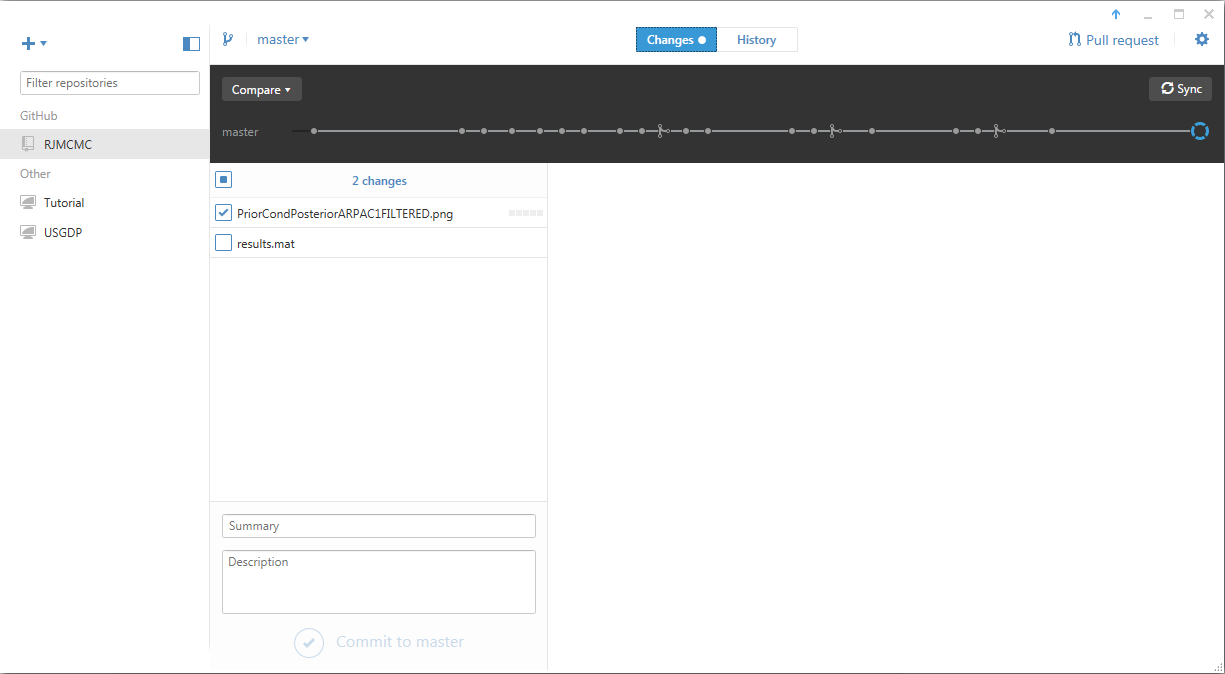
\includegraphics[height=0.6\textheight]{githubdesktop}
	\end{center}
}

\frame{
	\frametitle{Web Interface}
	\begin{center}
		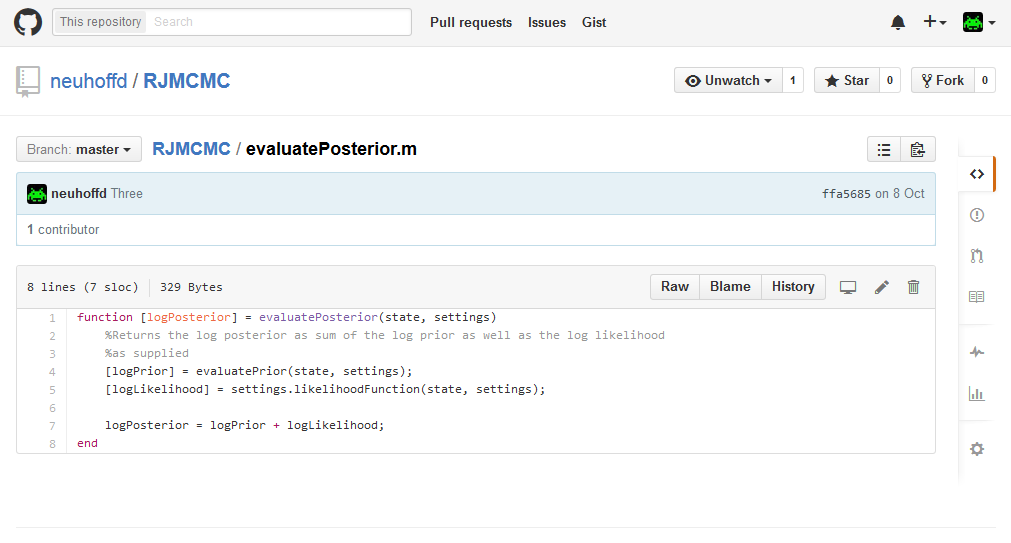
\includegraphics[height=0.6\textheight]{webinterface}
	\end{center}	
	
}

\frame{
	\frametitle{Command Line}
	\begin{center}
		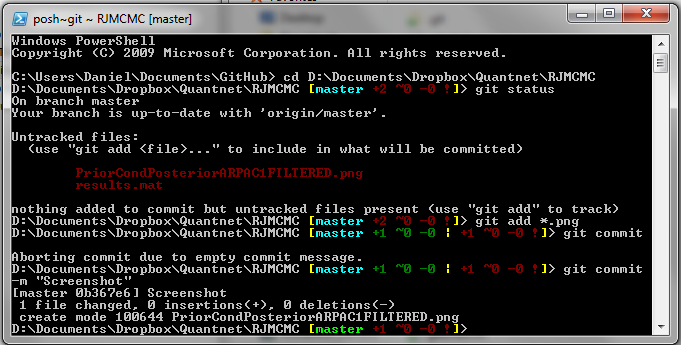
\includegraphics[height=0.6\textheight]{commandline}
	\end{center}		
}

\section{GitHub and QuantNet 2.0}

\frame{
	\frametitle{What I did}
	\begin{enumerate}
		\item Create GitHub repository
		\item Move code into GitHub repository
		\item Develop with an eye on style guidelines
		\item Write readme.md
		\item Declare running version ready for audit
	\end{enumerate}		
	
	After the audit is complete, the code is moved to a specific GitHub repository and appears on the QuantNet 2.0 page	
}

\frame{
	\frametitle{What else could one do?}
	\begin{itemize}
		\item Collaborate with other scientists around the world using the GitHub workflow
		\item Fork existing Quantlets in order to improve or extend them (ask the original author!!!!)
		\item Use Pulse and Graphs to track contributions and progress
		\item Use Milestones to structure a project
	\end{itemize}
}

 \frame{
 	\begin{center}
\textbf{Thank you for your attention!} 	
 	\end{center}

    }


% Adding an appendix for backup slides
\setcounter{figure}{0}
\setcounter{table}{0}
\appendix
\renewcommand{\thepage}{A-\arabic{page}}
\renewcommand{\theframenumber}{A-\arabic{framenumber}}
\renewcommand{\insertframenumber}{A-\arabic{framenumber}}
\renewcommand{\thefigure}{A-\arabic{figure}}
\renewcommand{\thetable}{A-\arabic{table}}
\renewcommand{\bibsection}{}


\begin{frame}[allowframebreaks]
   \frametitle{References}
   \bibliographystyle{../aea_doi_url_href}
   {\small \bibliography{D:/Documents/Dropbox/Dissertation/literaturegeneral}}
\end{frame}


\end{document}

